\documentclass{article}
\usepackage[utf8]{inputenc}
\usepackage{graphicx}
\usepackage[UKenglish]{babel}
\usepackage[margin = 1in]{geometry} %Remove for default margins
\usepackage{natbib}
\usepackage{mathtools}
\usepackage{siunitx}
\usepackage{url}
\usepackage{listings}
\usepackage{caption}
\usepackage{subcaption}

%TODO WHERE USED x change to X-Axis

\begin{titlepage}
    \title{Solar Simulation Experiment\\Computer Simulation Project 2019} 
    \author{Benjamin Carpenter (S1731178)}
    \date{7th March to 5th April 2019}
\end{titlepage}
\begin{document}
    \maketitle
    \addtocounter{page}{-1}
    \thispagestyle{empty}
    \pagebreak
    \pagestyle{empty} %get rid of header/footer for toc page
    \tableofcontents %put toc in
    \cleardoublepage %start new page
    \pagestyle{plain} % put headers/footers back on
    \setcounter{page}{1} %reset the page counter

    \section{Introduction \& Aims}
        This experiment would aim to simulate the motion of bodies within the inner solar system and to use this simulation to determine 
        if the Beeman algorithm would conserve total energy over time (as would be expected for a 
        simplified model of the solar system). The simulation would also be used to plot a course 
        for a probe from the surface of Earth to some distance close to Mars and determine if this 
        path could also allow for a return journey to Earth; this probe path would be compared to a
        probe path used by NASA's Viking mission\cite{VIKINGPROGRAMNASA}.
    
    \section{Theory used to simulate orbital motion}
        \subsection{The Gravitational force}
        Objects in space move due to gravity from other objects. This motion is dependent upon the 
        distances between objects as well as the masses of these objects, the force acting between 
        two objects of mass $m_1$ and $m_2$, with displacement $\vec{r}$ is given by:
        \begin{equation}
            \centering
            \vec{F} =-\frac{Gm_1m_2}{r^2}\hat{\textbf{r}}
            \label{eqn:GravitationalForce}
        \end{equation}
        \begin{flushright}
            From \cite[s. 3.12]{PHYS1ANOTES}
        \end{flushright}
        
        Where $G$ is a constant 
        $G = \num{6.67408e-11} \si{\metre}^3\si{\kilo\gram}^{-1}\si{\second}^{-2}$   
        \cite{GRAVCONST}   
        and  $\hat{\textbf{r}}$ is toward the other body as shown in fig.\ref{fig:GRAVFORCE}.
        
       
        \begin{figure}[!ht]
            \centering
            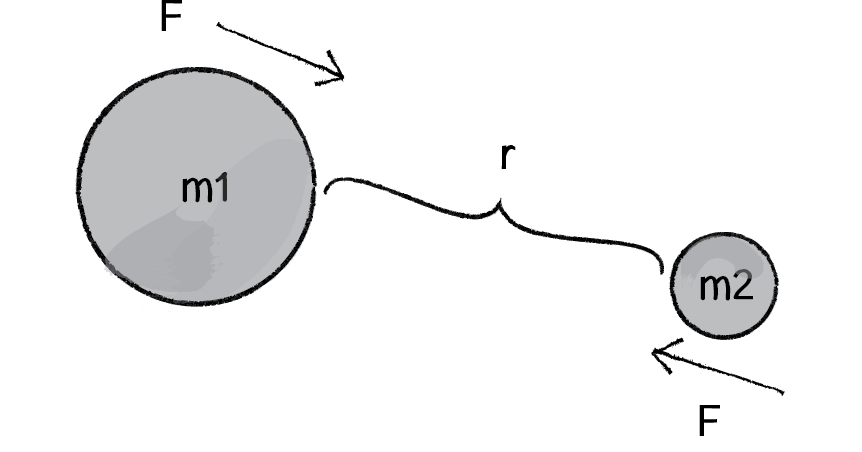
\includegraphics{Figures/GravitationalForce.png}
            \caption{Gravitational Force (\ref{eqn:GravitationalForce}) between two masses}
            \label{fig:GRAVFORCE}
            \cite{GravDiagram}
        \end{figure}

        \subsection{Potential and Kinetic Energies of objects moving in space}
            The kinetic energy of an object moving in space can be described simply from its mass $m$ 
            and speed $v$ in the relationship:
             \begin{equation}
                \centering
                E_{K} = \frac{1}{2}mv^2
                \label{eqn:KineticEnergy}
             \end{equation}
             \begin{flushright}
                 From \cite[s. 4.4]{PHYS1ANOTES}
             \end{flushright}

             \par
             Energy that a body stores due to its position relative to another body is given by the 
             integral of the magnitude of force (described in eqn \ref{eqn:GravitationalForce}) with respect to 
             position hence the relationship:
             \begin{equation}
                \centering
                E_P = \frac{Gm_1m_2}{r}
             \end{equation} 
             \begin{flushright}
                 From \cite[s. 4.6]{PHYS1ANOTES}
             \end{flushright}

             It should be noted that as this is a pair potential, if summing these energies for a 
             single object then the produced value should be halved to prevent 'double counting' 
             energies.


            %%%%%%%%%%%%%%%%%%%%%%MAYBE INCLUDE,MAYBE DONT, UNUSURE%%%%%%%%%%%%%%%%%%%%%%%%%%%%%% 
        %%%%\subsection{Numerical Integration - The three step Beeman scheme}
        %%%%     An accurate method to calculate position and velocity for an object at a time given its
        %%%%     acceleration is through usage of the three step Beeman scheme, this is giv

    \section{Implemented code and Experimental Method}
        \subsection{Overall interaction between objects}
            The main simulation was made up of three classes: A space object would contain within it 
            many body objects which would each represent a planet or other type of body (such as a 
            probe). An AnimateSpace class could then be used to either animate this space before or 
            after data for it had been processed.
            \par
            Two other minor classes were included in the program however these provide minimal 
            functionality:
            \par
            Probe develops on the body class adding features that would only be expected of a 
            controlled object (e.g. launching after two years as specified in experiment.3
            \cite[s. Solar 1.4.3]{CourseBook}).

            \par 
            Path acts as a storage structure to simplify interaction with data about
            a bodies path as it travels through space being used by \verb|Animatespace| to show 
            a bodies path.
            \par
            These interactions are summarised in fig.\ref{fig:classDiagram}.

        
        \begin{figure}[!ht]
            \centering
            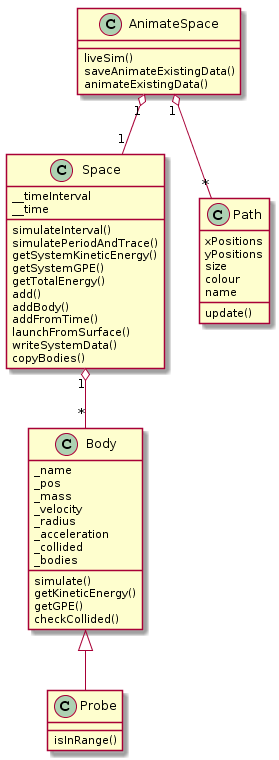
\includegraphics[width = 0.3\linewidth]{Figures/classDiagram.png}
            \caption{Class diagram of the main simulation files}
            \label{fig:classDiagram}
        \end{figure}

        \pagebreak
        \subsection{Bodies within space - The Body and Probe Class}
            This class is used to provide the properties of each body as well as being 
            responsible for updating these values when called to do so with the \verb|simulate| method. 
            Its properties also providing details to produce a representation in an animation as 
            shown in fig.\ref{fig:classDiagram}.
            
            \subsubsection{Simulating changes in position - The Beeman Integration method}\label{S:Accel}

                Each body would have a property which referenced the list of bodies stored 
                within the space object it was a part of; this was important as the motion of a body
                in space is dependent upon other masses that it is in contact with (see eqn 
                \ref{eqn:GravitationalForce}).

                \par 
                Being able to calculate this force allowed for an acceleration to be calculated, 
                simply by Newton's second law, this could hence be used with the Beeman integration 
                method to produce a new value for position and velocity which could then be used to 
                produce the next 'steps' force. 
                \par
                Applying this iteratively could simulate a bodies movement in space accurately. This 
                method required storing the acceleration of the body and required both a step back
                and forward acceleration at the same at the same time. 
                Usage of the various acceleration variables followed the algorithm show shown in 
                fig.\ref{fig:AccAlgorithm}, noting that \verb|__acceleration| is the only 
                property that is stored outside of the scope of this algorithm.
                \begin{figure}[!ht]
                    \centering
                    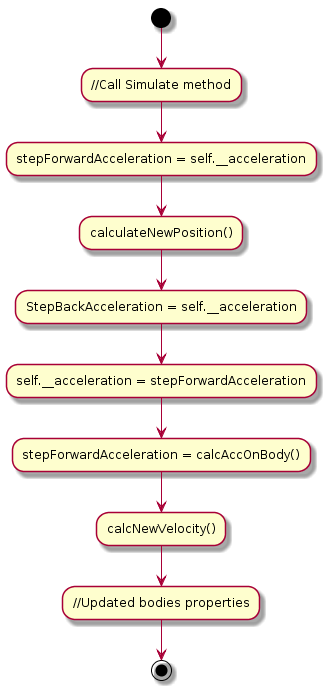
\includegraphics[width = 0.3\linewidth]{Figures/AccelerationAlgorithm.png}
                    \caption{Basic algorithm for updating the position and velocity.}
                    \label{fig:AccAlgorithm}
                \end{figure} 
                \par 
                \pagebreak
                It was expected that when calculating the 'step ahead' positions, the 'current
                position' was not to be updated, this would be expected to  have the effect of 
                adding a systematic error to each position where they were off-put due to not using 
                the correct position for a given interval ,therefore, a copy of the space objects
                \verb|__bodies| would be updated with the new positions which would have the effect
                of keeping the original property constant and removing the error. This copying would
                be done before an interval simulation i.e. where many bodies were being updated and
                hence was implemented in \verb|Space|.
                \par
                Unexpectedly, this had the effect of causing an apparent increase in energy, for 
                example, the orbits of planets would appear to increase as shown in fig.\ref{fig:DifferencesDueCopy}
                
                \begin{figure}[!b]
                    \centering
                    \begin{subfigure}{0.5\textwidth}
                        \centering
                        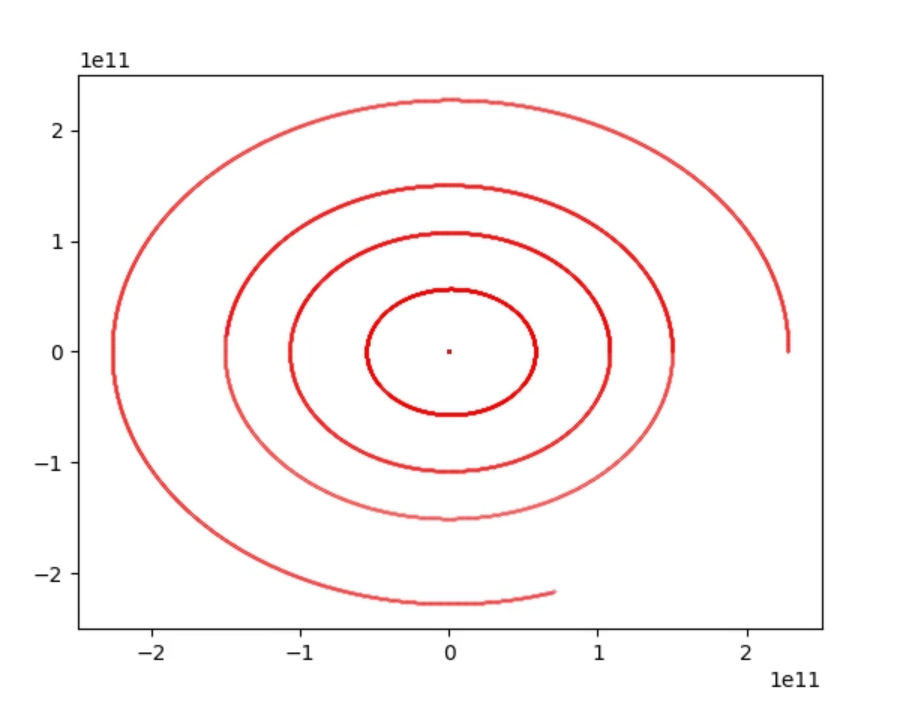
\includegraphics[width=\linewidth]{Figures/InnerPlanetsWhereCopyIsNotUsed.png}
                        \caption{Produced Graphic when using updated positions to \\calculate acceleration of a body in an iteration}
                        \label{subFig:nonCopy}
                    \end{subfigure}%
                    \begin{subfigure}{0.5\textwidth}
                        \centering
                        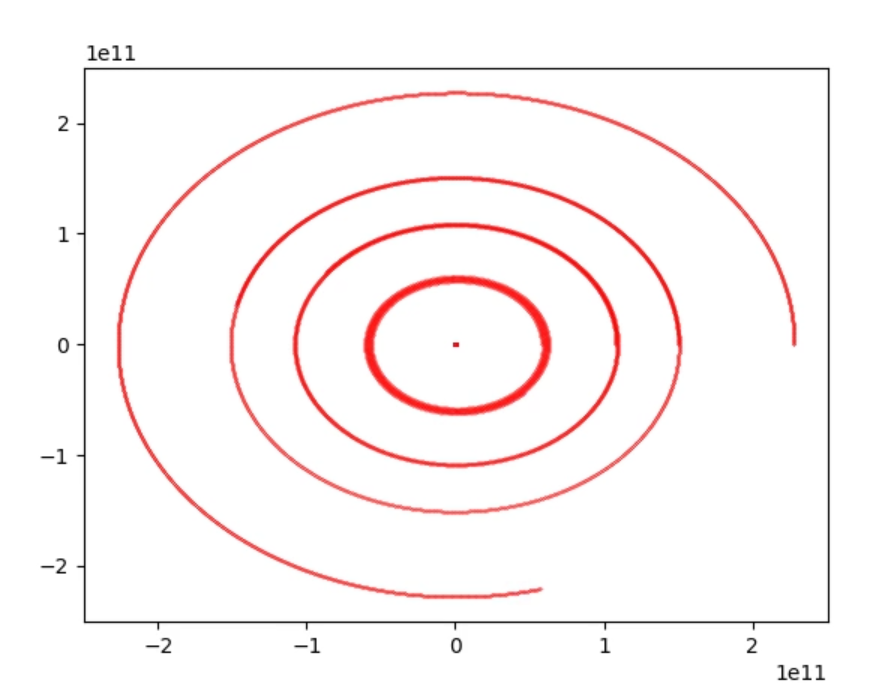
\includegraphics[width=1\linewidth]{Figures/InnerPlanetsWhereCopyIsUsed.png}
                        \caption{Produced Graphic when using non updated positions to calculate the acceleration of a body in an iteration}
                        \label{subFig:Copy}
                    \end{subfigure}    
                    
                    \caption{Apparent proper behaviour shown by algorithm that did not seem initially valid (i.e. deviation from a constant path is visible in \ref{subFig:Copy} due to wider path lines) }
                    \label{fig:DifferencesDueCopy}
                \end{figure}


                It was therefore decided that the bodies would not be copied at each interval and 
                instead would simply use the list of bodies as it was as this appeared to 
                produce the correct behaviour. This is further justified in appendix 
                \ref{App:FurtherImpDiscussion}.  %TODO ADD DATA TO FURTHER VERIFY THAT THIS IS AN OK ASSUMPTION TO MAKE !!!!!!!!!!!!!!!!!!!!!!!
            
          
                \pagebreak
            \subsubsection{Dealing with collisions} \label{S:collisionPro}
                A property to note was the boolean \verb|_collided| which record if a body had 
                collided with another (determined from if one body was at a distance that was within
                the distance of another plus its radius) afterwhich the simulation could not
                reliably simulate its behaviour due to loss of energies in the collision.
                \par 
                By marking these objects as collided experiments which were run using this program
                would be able to choose what should happen when a collision occurs rather than the 
                source program providing some action that may be inappropriate e.g. a tiny probe 
                colliding with the sun will have little effect to the system. Recording allows a
                specific behaviour to be implemented by the experimenter.
                \par 
                


            
            
        
        
        \subsection{The Programs simulation space - The Space Class}
                Acting as a container and controller for the bodies to be simulated in meant that 
                the \verb|Space| class would mostly contain functionality for making each body
                perform actions as well as collecting data about the entire system.
                \par 
                A representative method that showed this behaviour was the 
                \verb|simulatePeriodAndTrace| method which was used to generate simulation data of 
                the currently setup system (usually read in from file by the \verb|addFromFile| 
                method) over a given time and record the properties at each 'universal' time step. 
                This functionality would involve going through each body created in the \verb|Space| 
                object and simulating the time step for each separately (using their \verb|simulate|
                methods). Then the new body positions and properties could be recorded by 
                copying each body into a new list which would contain the changing bodies over time.

                \subsubsection{Generating data on bodies through simulation}
                Another core functionality of the \verb|Space| class was collecting data about the 
                system such as the  simulation time and values of gravitational potential and 
                Kinetic energies again this would work in general by iterating over each body and
                determining these properties for each and then combining these together
                 appropriately.

                \par
                The object was also able to generate a prediction for the stable orbital period of a
                body by calculating the time difference between the body in question being in the
                same position to within a fraction of the position change between intervals. 
                This accounted for both variation in a bodies path and non-simulated positions.

                \subsubsection{Launching from a body}
                    The \verb|Space| object allowed a body to be launched at the surface of another 
                    given a latitude and initial velocity. The body to be launched would be placed a 
                    distance slightly larger than the sum of radii of the launch object and body 
                    from their centers of mass to prevent an immediate collision.
                
        \subsection{Animating the produced data - The AnimateSpace Class}
        To produce an animated output of generated data the \verb|AnimateSpace| class was used, this
        was able to parse the data produced by a \verb|Space| object and output it in an animated 
        format (through use of the \verb|Matplotlib| library
        \cite{MatPlotLib}). 
        The class is able to run a simulation and immediately output it to the screen using the 
        \verb|liveSim| method or alternatively can be used to animate an existing data set as well
        as saving to file.
        \par 
        This came about due to it being easier to debug basic behaviour using the 'on the fly' 
        method however this became slow for large datasets and would not allow for easily reviewing 
        what had occurred in an animation hence the further methods were implemented.
  
        

        
        \subsection{Experimental Scripts to produce data}
            \subsubsection{Constant Total Energy} \label{S:ConstantTotalEnergyMethod}
                A script was created that would simply run a selection of bodies from file over a 
                given time period and output the energies as a graph as well as (as already required
                ) outputting the data to a file for further analysis using spreadsheet software. 
                This script provided a quick method for checking if energies were conserved after 
                making changes to the implementation.
            \subsubsection{Probe Path From Earth to Mars}\label{S:PathToMarsMethod}
                To determine a path between Earth and Mars a simple script was created to iterate 
                over the various possible launch parameters (latitude, initial Y-axis velocity and 
                initial X-axis velocity) and determine the closest position to Mars that was reached by
                the probe in a certain time frame as well as writing each result to file.
                \par
                To add some efficiencies to an otherwise very basic data collection script as well 
                as when meeting the decided stop time, the script would also stop simulating a 
                certain launch parameter when the \verb|_collision| property (discussed in section 
                \ref{S:collisionPro}) of the probe was \verb|True|.This generally
                meant that the probe had crashed into Earth or Mars (unfortunately more often and 
                less usefully Earth) which were conditions where no more useful data could 
                be collected.
                \par 
                This script could have been automated to rerun itself until optimal parameters were 
                found however it was more simple to run it multiple times focussing on 'close' 
                (i.e. smallest closest distance) values through interpretation of the data by hand
                than add this functionality. 
                \par
                By using this script many times, the range and intervals used could be reduced to a 
                point where a few 'good' (valid time and within a close distance i.e. a few 
                kilometres of Mars) paths generated. These could then be animated to see how they
                compared to known paths/each other. 
                \par 

                Through running an 'on the fly' animation, the time to intercept could then be 
                determined for each of the produced 'promising' results by stopping at intercept and
                getting the time from the output file.
        %%%\subsection{Data used in Experimentation}%%%TODO Discuss the data that was used in simulations 
    \pagebreak
    \section{Results \& Analysis}
        \subsection{Basic Program Functionality}
                The classes were usable to generate data and output this in an animated form, 
                examples of these are shown in fig.\ref{fig:AnimationExample}.
                \par
                These appeared to show the correct ratios between the different planets, 
                fig.\ref{subfig:MercuryVsWorld} shows Mercury has reached its orbital period of 
                 88days\cite{PlanetDat} whilst Venus is at around a third of its total orbital 
                 period (a Venus year is 243 Days\cite{PlanetDat}), hence the ratio of these two 
                 orbital periods is $\frac{88}{243} 0.36$ or just over a third of the total 
                 journey which is the visible distance covered in fig.\ref{subfig:MercuryVsWorld}. 
                 \par
                 We can also see that the ratio of Earth (where a year is 365.25 days) to Mercury 
                 appears to be around a quarter, this matches the ratio of orbital periods of 
                 $\sim 0.24$.
                \par
                We can see in fig.\ref{SubFig:MarsVsEarth}, Mars is about halfway through a Mars 
                year. This is the expected result from its year 687 Days vs Earth's 365.25 Days
                 (a ratio of $\sim 0.53$) \cite{MarsEarthData}

               
                \begin{figure}[!ht]
                    \centering
                    \begin{subfigure}{.5\textwidth}
                        \centering
                        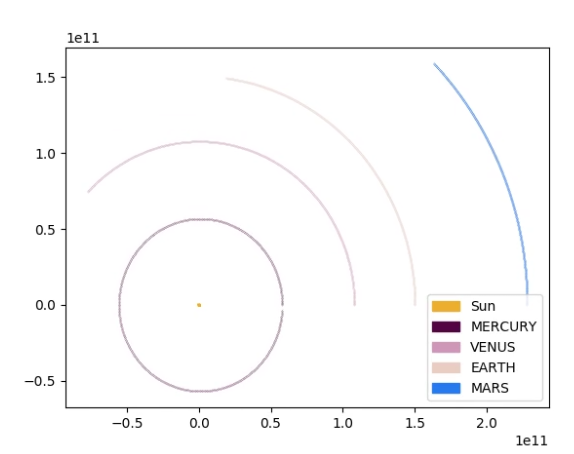
\includegraphics[width= 0.9\linewidth]{Figures/PreMercuryCompleteOrbit.png}
                        \caption{Animation just before completion of a Mercury year}
                        \label{subfig:MercuryVsWorld}
                        
                    \end{subfigure}%
                    \begin{subfigure}{.5\textwidth}
                        \centering

                        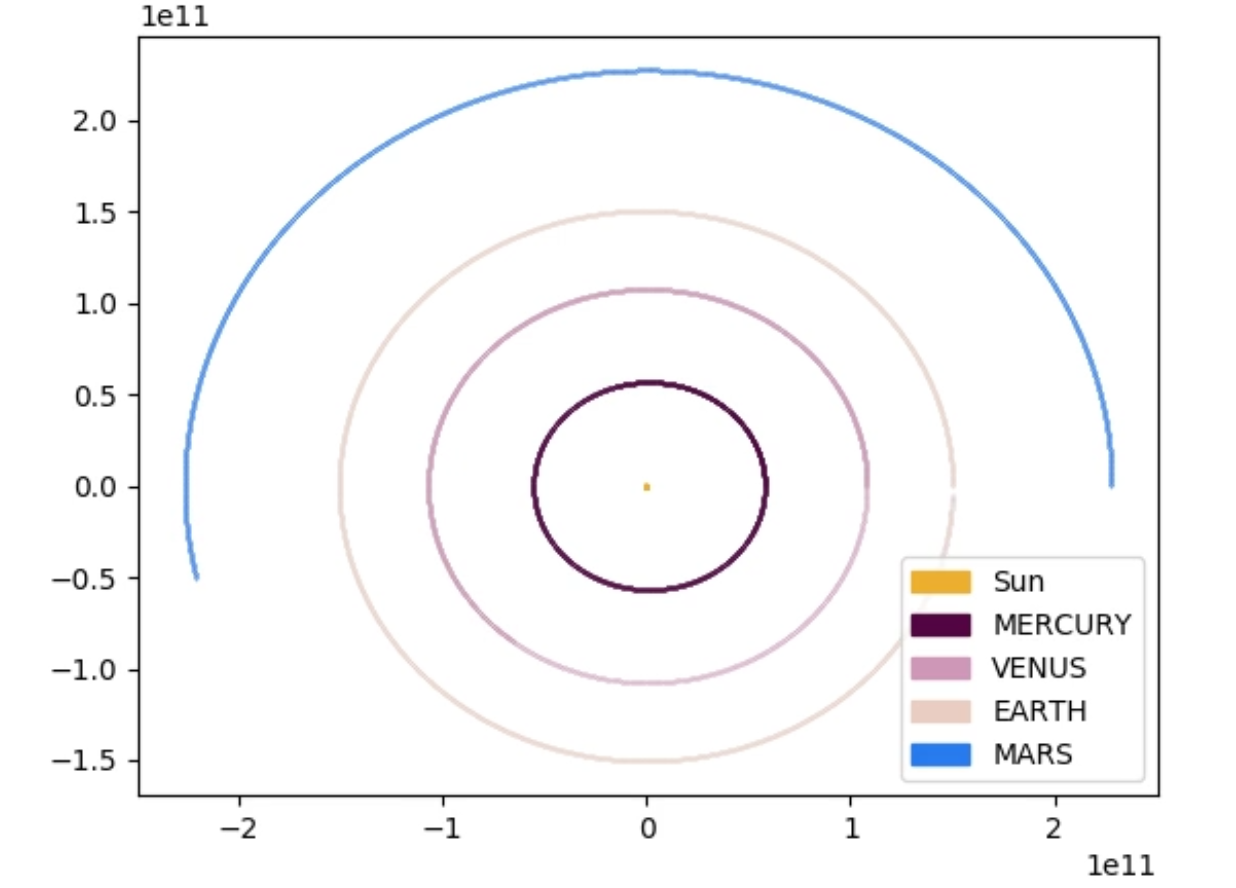
\includegraphics[width=\linewidth]{Figures/AnimatedExample1.png}
                        \caption{Animation just before an Earth year has passed}
                        \label{SubFig:MarsVsEarth}
                    \end{subfigure}
                    
                    \caption{Graphic showing stills from an animation of the inner planets of the 
                    solar system}
                    \label{fig:AnimationExample}    
                \end{figure}

                These visual ratios are also backed by the fact that the orbital periods of the
                planets matched their known values to within $5\%$ for all values and to within 
                $1\%$ for the majority as seen in fig.\ref{fig:prodLabel}.
                 
                \begin{figure}
                    \centering
                    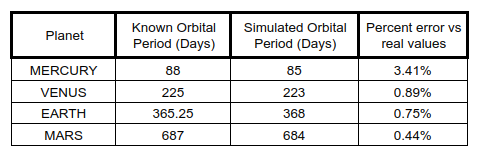
\includegraphics[width = 0.5\linewidth]{Figures/RatiosToRealValues.png}
                    \caption{Percentage error in known\cite{PlanetDat} and simulation produced
                    values for orbital period}
                    \label{fig:prodLabel}
                \end{figure}
                

            \pagebreak
            \subsection{Conservation of total energy within the system}
                By creating a simulation that simulated an overall time of 2 years (with an interval 
                of 1 hour) a collection of data points for the various energies in the system was 
                generated. These were then plotted to determine if energy was conserved over time, 
                this is shown in fig.\ref{fig:constEnergyProgOut}. 
                
                \begin{figure}[!ht]
                    \centering    
                    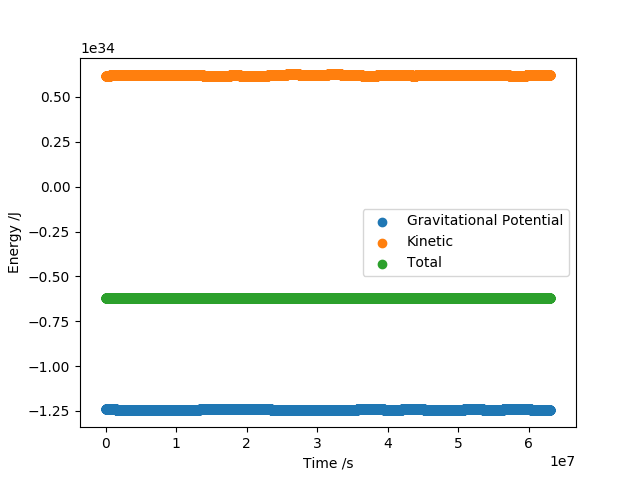
\includegraphics[width = 0.5\linewidth]{Figures/ConstEnergy/ConstEnergyPROGOUT.png}
                    \caption{Comparison of energies over time produced with the inner planets}
                    \label{fig:constEnergyProgOut}
                \end{figure}
                \pagebreak
                Using the outputted data with spreadsheet software the data could be better viewed 
                as well as allowing determination of uncertainty for data as seen in 
                fig.\ref{subFig:ConstEnergyGraph}. An appropriate uncertainty for 
                total energy was the propagation of uncertainties from Kinetic and Gravitational 
                potential energies. The uncertainty in each of which was used as standard
                deviation of the data describing the dispersion in values and hence an 
                appropriate uncertainty for the large data set. Looking closer at the data's
                trend (see fig.\ref{subFig:ConstEnergyNoUncertainty}) without uncertainty suggested 
                that it appeared that energy was decreasing with time, the uncertainty however made 
                this trend less well founded and hence could be disregarded further verified by 
                performing the test again over a larger time period
                (20 years) as seen in fig.\ref{subFig:ConstEnergy20Yr}.

                \begin{figure}[!ht]
                    \centering
                    \begin{subfigure}{0.5\textwidth}
                        \centering
                        \includegraphics[width =0.75\linewidth]{"Figures/ConstEnergy/Const energy Uncertainty".PNG}
                        \caption{Graph showing total energy vs time with\\ uncertainty}
                        \label{subFig:ConstEnergyGraph}
                    \end{subfigure}%
                    \begin{subfigure}{0.5\textwidth}
                        \centering
                        \includegraphics[width=0.75\linewidth]{"Figures/ConstEnergy/Const energy No Uncertainty".PNG}
                        \caption{Graph showing total energy vs time without \\uncertainty}
                        \label{subFig:ConstEnergyNoUncertainty}
                    \end{subfigure}
                    \begin{subfigure}{0.5\textwidth}
                        \centering
                        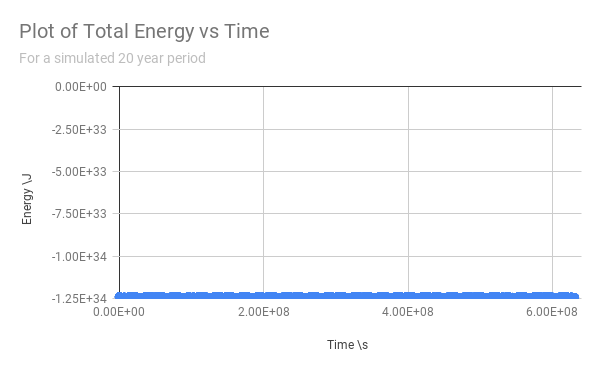
\includegraphics[width=0.75\linewidth]{Figures/ConstEnergy/ConstEnergy20yrs.png}
                        \caption{Energy vs time over a 20 year period showing an overall constant value}
                        \label{subFig:ConstEnergy20Yr}
                    \end{subfigure}
                    \caption{Figures showing constant energy vs time, ran using the inner planets.}
                \end{figure}


            \pagebreak
            \subsection{Plotting a path to Mars}
                The iterative approach of collecting a large collection of data for various 
                latitudes and launch velocities as discussed in s.\ref{S:PathToMarsMethod} appeared to 
                be somewhat successful, it was able to determine various 'promising' parameters that 
                could then be animated to view how viable they were in producing a path to Mars.
                \par
                Initial results suggested that latitudes were key to determining the best path 
                whilst various launch velocities effectively only added noise to results as seen in
                fig.\ref{fig:ProbeInitialDataSet}.
                
                
                \begin{figure}[!ht]
                    \centering
                    \begin{subfigure}{0.5\textwidth}
                        \centering
                        \includegraphics[width=0.8\linewidth]{"Figures/ProbePathData/Data Set 1/initalXVelocityResults".png}
                        \caption{Initial results on launch X-axis velocity vs closest\\ distance to Mars}
                        \label{subFig:initXVel}
                    \end{subfigure}%
                    \begin{subfigure}{0.5\textwidth}
                        \centering
                        \includegraphics[width =0.8\linewidth]{"Figures/ProbePathData/Data Set 1/initalYVelocityResults".png}
                        \caption{Initial results on launch Y-axis velocity vs closest distance to Mars}
                    \end{subfigure}%
                    \\
                    \begin{subfigure}{0.5\textwidth}
                        \centering
                        \includegraphics[width=\linewidth]{"Figures/ProbePathData/Data Set 1/initalLatitudeResults".png}
                        \caption{Initial results on launch latitude vs closest distance to Mars}
                        \label{subFig:initLat}
                    \end{subfigure}%

                    \caption{Effect of launch parameters on determining a path to Mars in the initial (and most general) data set collected}
                    \label{fig:ProbeInitialDataSet}
                \end{figure}


                \pagebreak

                As the range of angles that were being tested was reduced launch velocities became
                more important in determining the proper path to Mars as seen in fig.\ref{fig:Probe3rdDataSet}

                \begin{figure}[!ht]
                    \centering
                    \begin{subfigure}{0.4\textwidth}
                        \centering
                        \includegraphics[width=0.8\linewidth]{"Figures/ProbePathData/Launch x velocity vs Closest Distance (1)".png}
                        \caption{Trend in launch X-axis velocity vs closest \\distance. Visibly closest distances were\\ where X was close to $2600 \si{\meter \second^{-1}} $}

                    \end{subfigure}
                    \begin{subfigure}{0.4\textwidth}
                        \centering
                        \includegraphics[width=0.8\linewidth]{"Figures/ProbePathData/Launch Y Velocity vs Closest Distance (2)".png}
                        \caption{Trend in launch Y-axis velocity vs closest \\distance }
                    \end{subfigure}
                    \begin{subfigure}{0.6\textwidth}
                        \centering
                        \includegraphics[width=0.8\linewidth]{"Figures/ProbePathData/Launch Latitude vs Closest distance to Mars (2)".png}
                        \caption{Trend in launch latitude vs closest distance to Mars}
                    \end{subfigure}
                    \caption{Trends in launch parameters after three reductions in the range and intervals used}
                    \label{fig:Probe3rdDataSet}
                \end{figure}

                \pagebreak
                \par 
                The most realistic path produced was with the parameters:
                \begin{center}
                    \begin{tabular}{ll}
                        Latitude & $-50 \si{\degree}$\\
                        Initial X-axis velocity  & $10030\si{\meter \second ^{-1}}$\\
                        Initial Y-axis velocity &  $2525\si{\meter \second ^{-1}}$\\
                        Initial Speed & $10343\si{\meter \second ^{-1}}$
                        \label{tab:ParamUsed}
                    \end{tabular}
                \end{center}
                These related to intercept conditions of
                \begin{center}
                    \begin{tabular}{ll}
                        Intercept distance & $3.10\si{\kilo\meter}$ (i.e. a collision or landing)\\
                        Time to intercept & $2.5$ Months
                        \label{tab:ParamUsed}
                    \end{tabular}
                \end{center}
                
                This produced path is visualised in fig.\ref{fig:ProbeVisualisation}.
                \par
                The results of this path are unrealistic when compared to velocities that would be
                reasonable for usage with a probe as the time taken to reach the target of Mars is 
                much shorter than that of used paths such as that of the Viking mission which had 
                times to intercept of around 9 months \cite{VIKINGPROGRAMNASA}. 
                \par
                It is likely that the issue of an unrealistic orbit is due to 
                usage of only the most obvious intercepting launch parameters, from the large 
                collection of data produced by the initial run of the \verb|MarsProbeExperiment| 
                script, only $3$ of $\sim 4000$ data points were further investigated due to time
                constraints. It is likely therefore that investigation of other launch parameters 
                would yield more valid results. 
                \par
                Because this parameters overall speed was less than that of the Earth's escape 
                velocity $\sim 11\si{\kilo\meter \second^{-1}}$\cite{EarthEscapeVel} this would be 
                supportive that this method would likely able to through further analysis produce a 
                valid 'there and back again' path.

                
                \begin{figure}[!ht]
                    \centering
                    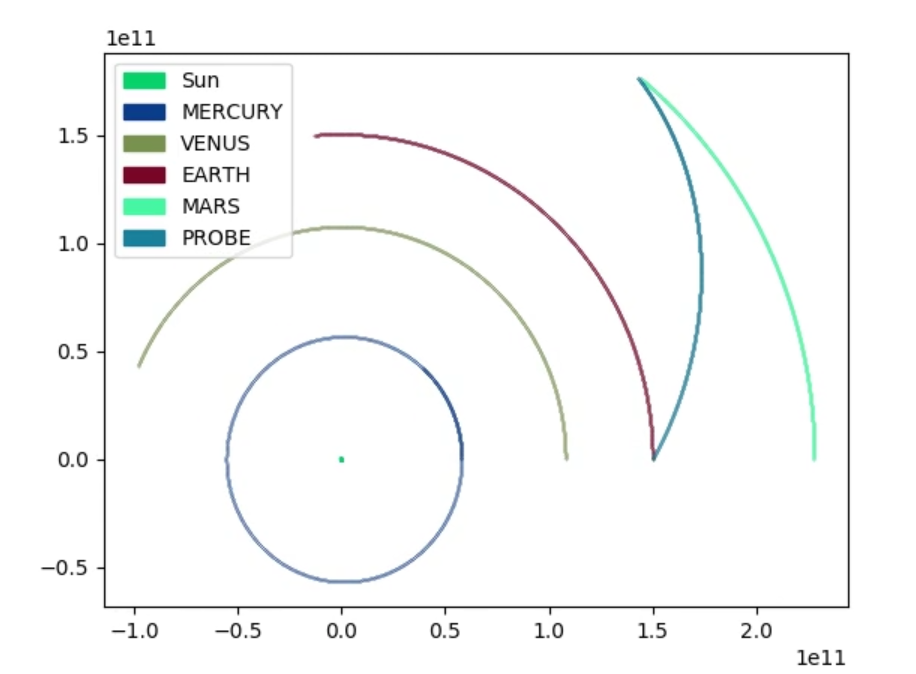
\includegraphics[width=0.5\linewidth]{Figures/ProbePathVisulisation.png}
                    \caption{Visualisation of a probe launched with parameters shown in \ref{tab:ParamUsed} .} 
                    \label{fig:ProbeVisualisation}
                \end{figure}

    \pagebreak       
    \section{Discussion on possible improvements}
        Overall this implementation was successful in simulating the movement of a 2D solar 
        system. Improvements could have been  added to the orbital period determination in ensuring 
        it was more accurate across all values types of planets as higher velocity bodies were 
        generally less realistic, as shown by Mercury in fig.\ref{fig:prodLabel}. This however, was an
        acceptable discrepancy for a planet which has a complex orbit \cite{MercuryOrbit}.

        The determination of probe paths could have been improved by considering a greater number 
        of experimental values either through automation of the process or simply given greater
        time to allow for testing of more launch parameters from the produced data sets. 


    \section{Conclusions of Experimentation}
    Overall this experimentation was able to produce results that would suggest a valid simulation of 
    the inner planets of the solar system. 
    \par
    It has shown valid ratios between planet's orbital periods as well as energy conservation 
    over time, as expected for a closed system.
    \par
    It was also usable to produce paths between Earth and Mars for a probe and although the paths 
    that were currently determined were not realistic for a probe, there was indication that a more 
    realistic path could be generated given further time for analysis.  
    
    \pagebreak
    \bibliographystyle{plain}
    \bibliography{biblography}
    \pagebreak
    \appendix
    \section{Further justification of implementation of simulating intervals method } \label{App:FurtherImpDiscussion}
    As discussed in section \ref{S:Accel} the current implementation does not copy the bodies before 
    calculating acceleration meaning that some bodies use an updated position whilst others do not.
    This decision was taken as it provided the expected output in various forms as already discussed.
    \par
    When testing the conservation of energy in the system it was found that when applying the 
    copying of data before calculating the acceleration the variation was much larger and not 
    covered by the uncertainty as shown in fig.\ref{fig:CopyEnergyOut}  further justifying the
    current implementation.

    \begin{figure}[h]
        \centering
        \includegraphics[width=0.5\linewidth]{"Figures/ConstEnergy/Const Energy Copy".PNG}
        \caption{Total Energy output shows a much larger variation versus
         that of the non 'copy bodies' implementation that is shown in fig.\ref{subFig:ConstEnergyGraph} 
         over the same period}
        \label{fig:CopyEnergyOut}
    \end{figure}
\end{document}